\documentclass[a4paper,12pt]{article}
\usepackage[utf8]{inputenc}
\usepackage[T1]{fontenc}
\usepackage[frenchb]{babel} % If you write in French
%\usepackage[english]{babel} % If you write in English
\usepackage{a4wide}
\usepackage{graphicx}
\usepackage{adjustbox}
\usepackage{placeins}
\usepackage{amsmath}
%\usepackage{minitoc}
%\usepackage{epstopdf}
%\usepackage [utf8]{inputenc}
%\usepackage [francais]{babel}
\usepackage {amsmath, amssymb}
%\usepackage {setspace}
\usepackage{enumerate}
%\usepackage{verbatim}
%\usepackage{tikz}
%\usepackage[a4paper]{geometry}
%\geometry{hscale=0.77,vscale=0.85,centering} 

\usepackage{float}
%\usepackage{slashbox}
%\usepackage{eurosym}
%
%\usepackage{fancyhdr}
%
%\usepackage{amssymb}
%
%\newcommand{\F}{\mathcal{F}}



\usepackage{listings}
\usepackage{color}


\begin{document}

%%%%%%%%%%%%%%%%%%
%%% First page %%%
%%%%%%%%%%%%%%%%%%

\begin{titlepage}
\begin{center}

\begin{center}
{\large   UNIVERSITY OF LIEGE \\
APPLIED SCIENCE FACULTY \\
Academic year 2017-2018}\\[0.5cm]
   \end{center} 


%\includegraphics[width=0.6\textwidth]{uliege-logo-couleurs-300}\\[1cm]


\vfill\noindent
% Title
\rule{\linewidth}{0.5mm} \\[0.4cm]
{ \huge \bfseries Information and coding theory \\ Project 3 \\[0.4cm] }
\rule{\linewidth}{0.5mm} \\[1.5cm]

% Author and supervisor
\noindent
\begin{center}
%\begin{minipage}{0.4\textwidth}
  %\begin{flushleft} 
  \large
    Damien \textsc{Seron}
  %\end{flushleft}
%\end{minipage}%

\end{center}


\vfill

% Bottom of the page
{\large  april 2018}

\end{center}
\end{titlepage}


\section*{4}
The first step of the implementation is to build the binary tree corresponding to the given probabilities. First, the probabilities are sorted in ascending order and given a number depending on their position (from 1 to N where N is the number of probabilities in the given vector). Then at each iteration the two smaller probabilities are removed and their sum is added to the list of probabilities with a number (previous largest number attributed + 1). In the adjacency matrix a way from the sum to the removed probabilities is added. The list of probabilities is sorted and a new iteration begins until only 1 probability is left in the list. 

In the resulting adjacency matrix every node can access precisely 0 or 2 other nodes, making it a representation of a binary tree. In order to give a code to each probability a recursive algorithm  will be applied in depth, starting with the root (last line of the matrix). At each call of the function on a node the child with the smallest number will see its code be (code of the current node + "0") and the child with the largest number will see its code be (code of the current node + "1"). Then the function is called recursively for each child.\\ ~\\

Here is an example of the code and tree generated.

\begin{table}[!h]
\begin{center}
\begin{tabular}{|c|c|c|c|c|c|c|c|c|}

\hline 
Probability  & 0.05  & 0.1 & 0.3 & 0.1 & 0.25 & 0.1 & 0.03 & 0.07 \\ 
\hline 
Associated code & 11111 & 010 & 10 & 011 & 00 & 110 & 11110 & 1110 \\ 
\hline 
\end{tabular}
\caption{Probabilities and associated codes generated by the function} 
\end{center}
\end{table}

Note : As seen in Figure 1, the orientation of the edges of the tree is from the greater probability to the smallest. This is the representation in the adjacency matrix but in the theoretical course we most often see the edges directed towards the root of the tree instead of the leaves (I tried this way but the visualisation of the tree was not well organised). The length of the code associated with a probability is the depth of the node corresponding to this probability, a smaller probability must have a depth $\geq$ than the depth of a greater probability. 

\begin{figure} [h!]
\begin{center}
  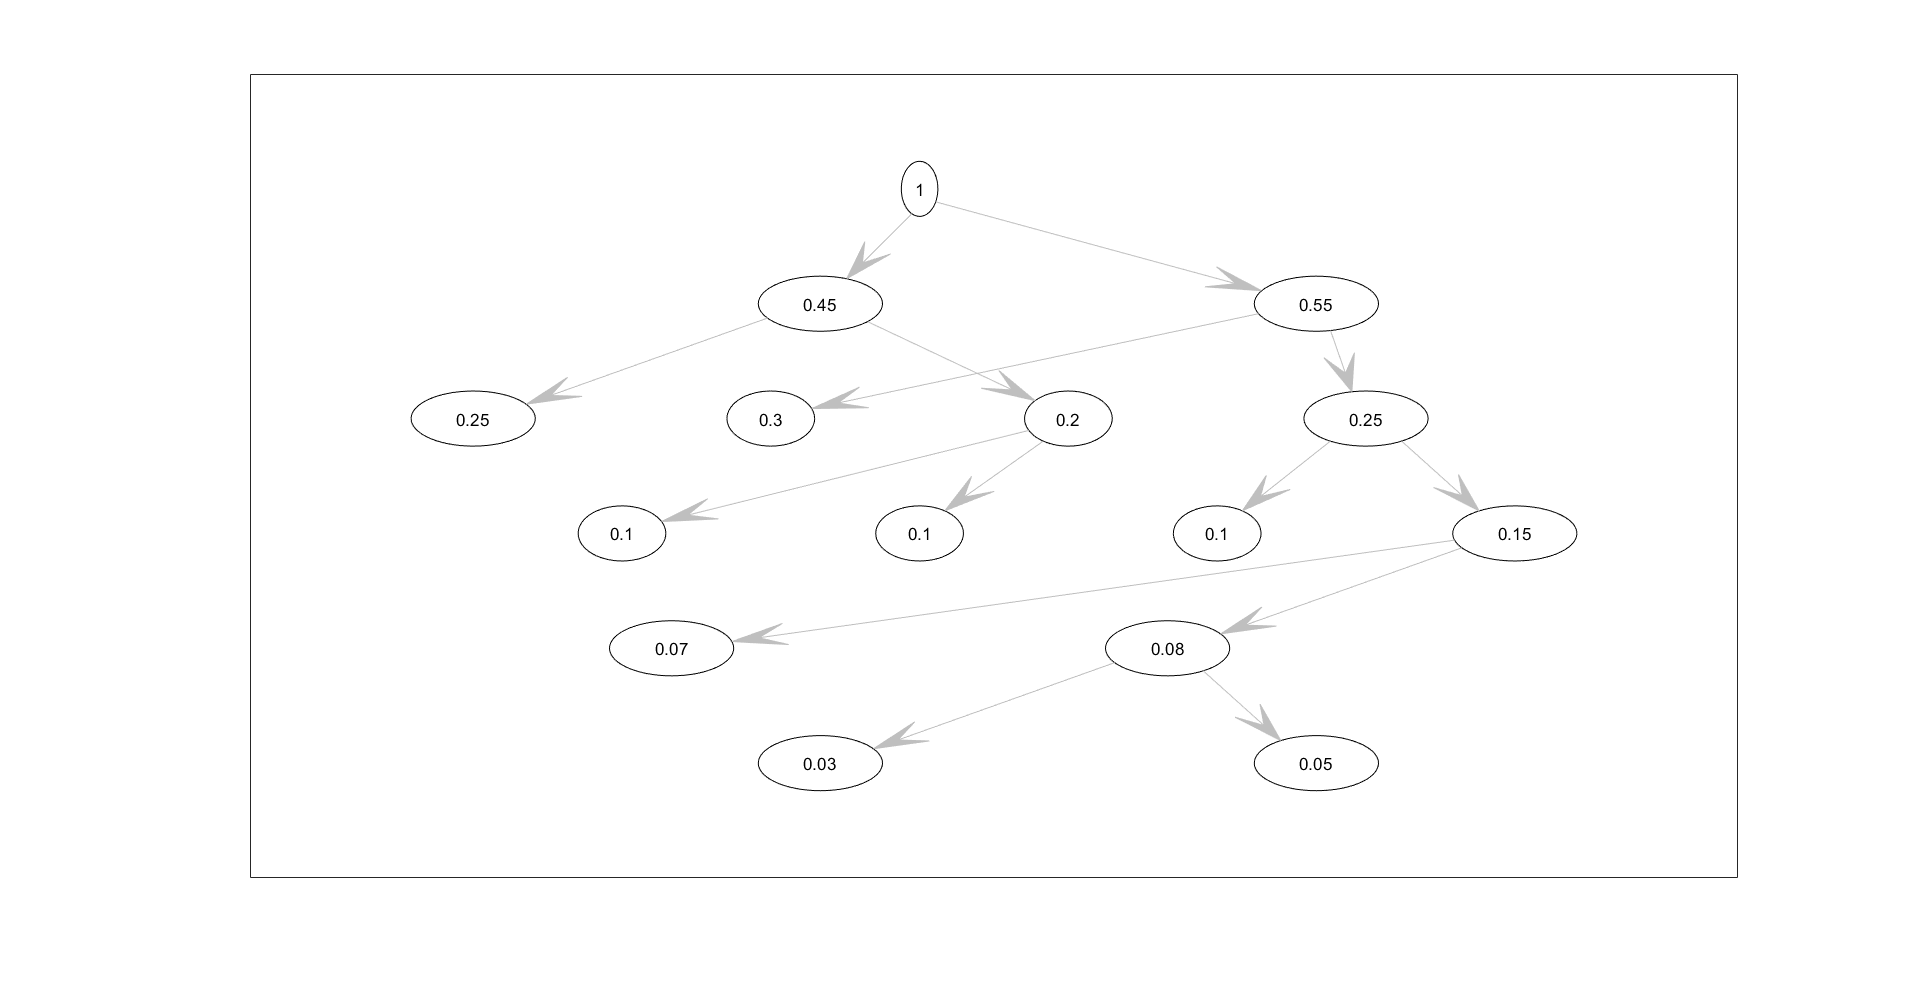
\includegraphics[scale=0.25]{large2.png}
  \caption{Visual representation of the adjacency matrix obtained with \textit{Huffman}. Each node is associated with a probability. The leaves are the probabilities given as argument. Each internal node is the sum of its children}
  \label{fig:--}
 \end{center}
\end{figure}

\section*{5}
The English alphabet is larger than the alphabet encountered in the text sample (Latin). It can still be used as every Latin letter can be found in the English alphabet but letters such as "j","k","w","y" and "z" will always have a probability of appearance of 0 since they do not exist in Latin.

\section*{6}
We could maybe, knowing how Latin works, have an alphabet with words such as "um" "us" and common declinations since those groups of letters can be quite frequent.

\section*{7}
We could model the source with an alphabet and the associated probabilities but also as a Markov chain with each time the probability of having a specific letter depending of the knowledge of the previous letter(s). If we take only into account the previous letter we have a transition matrix of size N x N (N is the alphabet size).  
\section*{8}
Each symbol is of length n = 4. In the data we only encounter Q = 16 distinct words and we know that q = 10 from the statement. 
\begin{equation}
\sum_{i=1}^{16} 10^{-4} = 1.6*10^{-3} \leq 1
\end{equation} 
The Kraft condition is respected. This means that there exists a uniquely decodable code having a length of 4 (with an alphabet from 0 to 9).
If we compute the probability of occurrence of each symbol with \textit{estimate\_proba} and then compute the entropy we obtain 3.6517. This is the optimal average length for a symbol (in bits). This code is not complete since the result of the sum in Kraft's inequality is not exactly 1.

\section*{9}
To represent a number in 0-9 we need at least 4 bits. To represent 4 numbers (one symbol) we then need 16 bits. With \textit{encode\_to\_numerals} we get codes between 1-16, which can be represented with 4 bits (starting with the value 1 and not 0). The resulting code is then 16/4 = 4 times compressed (compression rate of 4). Since we only detect 16 symbols in data we can expect after the use of \textit{encode\_to\_numerals} to receive a symbol of maximum 4 bits.
\begin{table}[h!]

\begin{center}

\begin{adjustbox}{max width=\linewidth}
\begin{tabular}{|c|c|c|c|c|c|c|c|c|c|c|c|c|c|c|c|c|}
 \hline 
 Symbol from the source & 1111 & 1112 & 1121 & 1122 & 1211 & 1212 & 1221 & 1222 \\ 
 \hline 
 Probability & 0.0083 & 0.00283 & 0.0550 & 0.09 & 0.0958 & 0.0042 & 0.0108 & 0.0908  \\ 
 \hline 
 Code  & 1 & 2 & 3 & 4 & 5 & 6 & 7 & 8 \\ 
 \hline 
\end{tabular}
\end{adjustbox}

\begin{adjustbox}{max width=\linewidth}
\begin{tabular}{|c|c|c|c|c|c|c|c|c|c|c|c|c|c|c|c|c|}
 \hline 
 Symbol from the source & 2111 & 2112 & 2121 & 2122 & 2211 & 2212 & 2221 & 2222 \\ 
 \hline 
 Probability  & 0.0875 & 0.1233 & 0.0958 & 0.0125 & 0.0325 & 0.1 & 0.0633 & 0.1017 \\ 
 \hline 
 Code & 9 & 10 & 11 & 12 & 13 & 14 & 15 & 16 \\ 
 \hline 
\end{tabular}
\end{adjustbox}
\end{center}
\caption{Symbols from the source with their probabilities of occurrence and their associated Huffman code}  
\end{table} 


\section*{10} 
Length of symbol n = 1, Q = 16 different messages encountered, q = 16 (the alphabet is a number between 1 and 16 represented with 4 bits)

\begin{equation}
\sum_{i=1}^{16} 16^{-1} = 1
\end{equation} 
This code is decodable, complete, regular, instantaneous and prefix-free (all codes are 4 bits sized and each one is associated with one symbol. No code is the prefix of the other -> prefix-free and instantaneous). This code is not absolutely optimal since the average symbol length is 1.
\begin{equation}
\overline{n} \neq \frac{H(S)}{log(q)} = 0.9129
\end{equation} 

\section*{11}

\begin{table}[h!]

\begin{center}

\begin{adjustbox}{max width=\linewidth}
\begin{tabular}{|c|c|c|c|c|c|c|c|c|}
\hline 
Probability & 0.0058 & 0.0278 & 0.0547 & 0.085 & 0.1065 & 0.0050 & 0.0108 & 0.0971 \\ 
\hline 
Code (binary) & 10111111 & 10110 & 0011 & 1101 & 011 & 10111110 & 1011110 & 010 \\ 
\hline 
\end{tabular}
\end{adjustbox} 

\begin{adjustbox}{max width=\linewidth}
\begin{tabular}{|c|c|c|c|c|c|c|c|c|}
\hline 
Probability & 0.0957 & 0.1285 & 0.08 & 0.0142 & 0.0422 & 0.0916 & 0.00592 & 0.0959 \\ 
\hline 
Code (binary) & 1111 & 100 & 1100 & 101110 & 0010 & 1110 & 1010 & 000 \\ 
\hline 
\end{tabular}
\end{adjustbox}
\end{center} 
\caption{Symbols from the source with their theoretical probabilities of occurrence and their associated Huffman code}  
\end{table}

The expected symbol length (theoretical probabilities) is
\begin{equation}
\sum_{i=1}^{16} p_i n_i = 3.7038
\end{equation}
Where $p_i , n_i$ are respectively the probabilities of occurrence of a symbol and the length of that symbol.
The compression rate is $\frac{16}{3.7038} = 4.3199$. 

\section*{12 - 13}

\begin{table}[h!]

\begin{center}

\begin{adjustbox}{max width=\linewidth}
\begin{tabular}{|c|c|c|c|c|c|c|c|c|c|c|c|c|c|c|c|c|}
 \hline 
 Symbol from the source & 1111 & 1112 & 1121 & 1122 & 1211 & 1212 & 1221 & 1222 \\ 
 \hline 
 Probability (from sample) & 0.0083 & 0.00283 & 0.0550 & 0.09 & 0.0958 & 0.0042 & 0.0108 & 0.0908  \\ 
 \hline 
 Code (binary) & 1111101 & 10110 & 11110 & 1101 & 000 & 1111100 & 1111110 & 1110  \\ 
 \hline 
\end{tabular}
\end{adjustbox}

\begin{adjustbox}{max width=\linewidth}
\begin{tabular}{|c|c|c|c|c|c|c|c|c|c|c|c|c|c|c|c|c|}
 \hline 
 Symbol from the source & 2111 & 2112 & 2121 & 2122 & 2211 & 2212 & 2221 & 2222 \\ 
 \hline 
 Probability (from sample) & 0.0875 & 0.1233 & 0.0958 & 0.0125 & 0.0325 & 0.1 & 0.0633 & 0.1017 \\ 
 \hline 
 Code (binary) & 1100 & 100 & 001 & 1111111 & 10111 & 010 & 1010 & 011 \\ 
 \hline 
\end{tabular}
\end{adjustbox}
\end{center}
\caption{Symbols from the source with their encountered probabilities of occurrence and their associated Huffman code}  
\end{table}


The obtained code is decodable, regular, instantaneous and prefix-free (Huffman encoding guaranties  prefix-free (and thus instantaneous) codes). If we check Kraft's inequality with $n_i \in [3;4;5;7]$(5 words of n = 3, 4 words of n = 4, 3 words of n = 5, 4 words of length n = 7) , Q = 16, q = 2 :
\begin{equation}
5 * 2^{-3} + 4 * 2^{-4} + 3 * 2^{-5} + 4 * 2^{-7} =  1
\end{equation}
We can see that the code is complete. The code is not absolutely optimal, if we do :

\begin{equation}
\sum_{i=1}^{16} p_i n_i = 3.7067 \geq \frac{H(S)}{log(q)} = 3.6517
\end{equation} 
We see that the average length (3.7067) is still superior to the optimal average length of a symbol $\frac{H(S)}{log(q)}$.

If we compare the resulting Huffman's encoding with question 11 we see that both codes are decodable, complete, regular, instantaneous and prefix-free but Huffman's encoding produces a smaller average length per symbol and is thus closer to the absolutely optimal average length. 

\end{document}
